In the previous chapter we introduced the compound criteria comprising minimisation of the model estimates' variation and bias arising from the potential model misspecification of a known form, together with the minimising the associated lack-of-fit. We considered an example of a factorial experiment and examined how the criteria would work in terms of the resulting optimal designs and the relationships between the individual components in terms of the relationships between the weight allocations and designs' performances.

A natural extension to be implemented in this chapter is to adapt the developed criteria to an other widely used experimental  framework, blocked experiments. Here we also consider a real-life example of a blocked experiment and provide some practical solutions for the experimenters according to the particular case-specific aims, objectives and restrictions.

\section{MSE-Based Criteria Adapted for Blocked Experiments}

We will start by reviewing the `full' model for blocked experiments, similar to (\ref{eq::blocked_model}):
\begin{align*}
\bm{Y}=\bm{Z\beta}_{B}+\bm{X}_{1}\bm{\beta}_{1}+\bm{X}_{2}\bm{\beta}_{2}+\bm{\varepsilon}.
\end{align*}
Denote the $n\times(b+p)$ model matrix of the block and primary terms by $\tilde{\bm{X}}_{1}=[\bm{Z},\bm{X}_{1}]$, where the columns of $\bm{Z}$ contain block indicators, and the columns of $\bm{X}_{1}$ correspond to primary terms. Let also $\bm{\tilde{\beta}}_1=[\bm{\beta}_{B},\bm{\beta}_{1}]'$ be the joint vector of fixed block effects and primary model terms, and by $\bm{\hat{\tilde{\beta}}}_1$ we denote the vector of the corresponding estimates. It is worth noting that the number of primary terms $p$ does not include the intercept, as it is aliased with the block effects.

%The $DP$-, $LP$- and $LoF(DP)$- and $LoF(LP)$-components are derived as was shown in Section \ref{sec::gen_blocked}.
Then the overall mean square error matrix is
\begin{align}
\label{eq::MSE_b}
\mbox{MSE}(\bm{\hat{\tilde{\beta}}}_1|\bm{\tilde{\beta}})=&\mathtt{E}_{\bm{Y}|\bm{\beta}}[(\bm{\hat{\tilde{\beta}}}_1-\bm{\tilde{\beta}}_1)(\bm{\hat{\tilde{\beta}}}_1-\bm{\tilde{\beta}}_1)'] \notag\\=&\sigma^2(\bm{\tilde{X}}_1^{'}\bm{\tilde{X}}_1)^{-1}+\bm{\tilde{A}}\bm{\beta}_2\bm{\beta}_2'\bm{\tilde{A}}', 
\end{align}
where $\bm{\tilde{A}}=(\bm{\tilde{X}}_1^{'}\bm{\tilde{X}}_1)^{-1}\bm{\tilde{X}}_1^{'}\bm{X}_2$ is the alias matrix in the case of a blocked experiment.

Now consider the partition of the MSE matrix with respect to block and primary effects:
\begin{align}
\label{eq::mse_b_matrix}
&\mathtt{E}_{\bm{Y}|\bm{\beta}}[(\bm{\hat{\tilde{\beta}}}_1-\bm{\tilde{\beta}}_1)(\bm{\hat{\tilde{\beta}}}_1-\bm{\tilde{\beta}}_1)']= \notag\\ &\mathtt{E}_{\bm{Y}|\bm{\beta}}\{[\hat{\tilde{\beta}}_{11}-\tilde{\beta}_{11},\ldots,
\hat{\tilde{\beta}}_{1b}-\tilde{\beta}_{1b}, \hat{\tilde{\beta}}_{1 b+1}-\tilde{\beta}_{1 b+1},\ldots, \hat{\tilde{\beta}}_{1 b+p}-\tilde{\beta}_{1 b+p}]\times \notag\\ &[\hat{\tilde{\beta}}_{11}-\tilde{\beta}_{11},\ldots,
\hat{\tilde{\beta}}_{1b}-\tilde{\beta}_{1b}, \hat{\tilde{\beta}}_{1 b+1}-\tilde{\beta}_{1 b+1},\ldots, \hat{\tilde{\beta}}_{1 b+p}-\tilde{\beta}_{1 b+p}]'\}=\notag\\
&\mathtt{E}_{\bm{Y}|\bm{\beta}}\{[\bm{\hat{\beta}}_B-\bm{\beta}_B, \bm{\hat{\beta}}_1-\bm{\beta}_1][\bm{\hat{\beta}}_B-\bm{\beta}_B, \bm{\hat{\beta}}_1-\bm{\beta}_1]'\}=\notag\\
&\begin{bmatrix}
\mathtt{E}_{\bm{Y}|\bm{\beta}}(\bm{\hat{\beta}}_B-\bm{\beta}_B)(\bm{\hat{\beta}}_B-\bm{\beta}_B)' & \mathtt{E}_{\bm{Y}|\bm{\beta}}(\bm{\hat{\beta}}_B-\bm{\beta}_B)(\bm{\hat{\beta}}_1-\bm{\beta}_1)'\\
\mathtt{E}_{\bm{Y}|\bm{\beta}}(\bm{\hat{\beta}}_1-\bm{\beta}_1)(\bm{\hat{\beta}}_B-\bm{\beta}_B)' & \mathtt{E}_{\bm{Y}|\bm{\beta}}(\bm{\hat{\beta}}_1-\bm{\beta}_1)(\bm{\hat{\beta}}_1-\bm{\beta}_1)'
\end{bmatrix}.
\end{align}

The $[2,2]$-submatrix (bottom-right) represents the entity we are interested in -- the bias of the estimators of the primary terms. Denote it by $\mbox{MSE}(\bm{\hat{\tilde{\beta}}}_1|\bm{\tilde{\beta}})_{22}$. Then the corresponding submatrix of the first summand in (\ref{eq::MSE_b}) is
\begin{equation*}
[\sigma^2(\bm{\tilde{X}}_1^{'}\bm{\tilde{X}}_1)^{-1}]_{22}=\sigma^2(\bm{X}'_{1}
\bm{QX}_{1})^{-1}, \mbox { where } \bm{Q}=\bm{I}-\bm{Z}(\bm{Z}'\bm{Z})^{-1}\bm{Z}'. 
\end{equation*}

Using the matrix inversion rule for block matrices \citep{Harville2006matrix}:
\begin{align*}
\begin{bmatrix}
\bm{A} & \bm{B}\\
\bm{C} & \bm{D}
\end{bmatrix}
^{-1}=
\begin{bmatrix}
(\bm{A}-\bm{BD}^{-1}\bm{C})^{-1} & -(\bm{A}-\bm{BD}^{-1}\bm{C})^{-1}\bm{BD}^{-1} \\
-\bm{D}^{-1}\bm{C}(\bm{A}-\bm{BD}^{-1}\bm{C})^{-1} & \bm{D}^{-1}+\bm{D}^{-1}\bm{C}(\bm{A}-\bm{BD}^{-1}\bm{C})^{-1}\bm{BD}^{-1}
\end{bmatrix},
\end{align*}

under the conditions of invertability of $\bm{A}$, $\bm{D}$ and $\bm{A}-\bm{BD}^{-1}\bm{C}$, we now consider $\bm{\tilde{A}}$:
\begin{align*}
\bm{\tilde{A}}=&\left(
\begin{bmatrix}
\bm{Z}'\\
\bm{X}'_{1}
\end{bmatrix}
\begin{bmatrix}
\bm{Z} & \bm{X}_{1}
\end{bmatrix}\right)^{-1}
\begin{bmatrix}
\bm{Z}'\\
\bm{X}'_{1}
\end{bmatrix}\bm{X}_{2}=
\begin{pmatrix}
\bm{Z}'\bm{Z} & \bm{Z}'\bm{X}_{1}\\
\bm{X}'_{1}\bm{Z} & \bm{X}'_{1}\bm{X}_{1}
\end{pmatrix}^{-1}
\begin{bmatrix}
\bm{Z}'\\
\bm{X}'_{1}
\end{bmatrix}\bm{X}_{2}=
\\ &
\begin{bmatrix}
(\bm{Z}'\bm{PZ})^{-1} & -(\bm{Z}'\bm{PZ})^{-1}\bm{Z}'\bm{X}_{1}(\bm{X}'_{1}\bm{X}_{1})^{-1} \\
-(\bm{X}'_{1}\bm{QX}_{1})^{-1}\bm{X}'_{1}\bm{Z}(\bm{Z}'\bm{Z})^{-1} & (\bm{X}'_{1}\bm{QX}_{1})^{-1}
\end{bmatrix}
\begin{bmatrix}
\bm{Z}'\\
\bm{X}'_{1}
\end{bmatrix}\bm{X}_{2}=\\ &
\begin{bmatrix}
(\bm{Z}'\bm{PZ})^{-1}\bm{Z}'\bm{PX}_{2}\\
(\bm{X}'_{1}\bm{QX}_{1})^{-1}\bm{X}'_{1}\bm{QX}_{2}
\end{bmatrix}, 
\end{align*}
where $\bm{P}=\bm{I}-\bm{X}_{1}(\bm{X}'_{1}\bm{X}_{1})^{-1}\bm{X}'_{1}$ is symmetric.

Here $\bm{ZZ}'$, $\bm{X}'_{1}\bm{X}_{1}$ and $\bm{Z}'\bm{PZ}$ are all invertible and, therefore, the operations are legitimate. 

Now consider the second summand in (\ref{eq::MSE_b}):
\begin{align*}
&\bm{\tilde{A}}\bm{\beta}_2\bm{\beta}_2'\bm{\tilde{A}}'=
\begin{bmatrix}
(\bm{Z}'\bm{PZ})^{-1}\bm{Z}'\bm{PX}_{2}\bm{\beta}_2 \\
(\bm{X}'_{1}\bm{QX}_{1})^{-1}\bm{X}'_{1}\bm{QX}_{2}\bm{\beta}_2
\end{bmatrix}
\begin{bmatrix}
\bm{\beta}'_2\bm{X}'_{2}\bm{PZ}(\bm{Z}'\bm{PZ})^{-1} & \bm{\beta}'_2\bm{X}'_{2}\bm{QX}_{1}(\bm{X}'_{1}\bm{QX}_{1})^{-1}
\end{bmatrix}=\\
&\begin{bmatrix}
(\bm{Z}'\bm{PZ})^{-1}\bm{Z}'\bm{PX}_{2}\bm{\beta}_2\bm{\beta}'_2\bm{X}'_{2}\bm{PZ}(\bm{Z}'\bm{PZ})^{-1} & (\bm{Z}'\bm{PZ})^{-1}\bm{Z}'\bm{PX}_{2}\bm{\beta}_2\bm{\beta}'_2\bm{X}'_{2}\bm{QX}_{1}(\bm{X}'_{1}\bm{QX}_{1})^{-1} \\
(\bm{X}'_{1}\bm{QX}_{1})^{-1}\bm{X}'_{1}\bm{QX}_{2}\bm{\beta}_2\bm{\beta}'_2\bm{X}'_{2}\bm{PZ}(\bm{Z}'\bm{PZ})^{-1} & (\bm{X}'_{1}\bm{QX}_{1})^{-1}\bm{X}'_{1}\bm{QX}_{2}\bm{\beta}_2\bm{\beta}'_2\bm{X}'_{2}\bm{QX}_{1}(\bm{X}'_{1}\bm{QX}_{1})^{-1}
\end{bmatrix}.
\end{align*}

Therefore, the submatrix of (\ref{eq::MSE_b}) corresponding to the primary terms is
\begin{align}
\label{eq::mesb_submatrix}
\mbox{MSE}(\bm{\hat{\tilde{\beta}}}_1|\bm{\tilde{\beta}})_{22}=&\sigma^2(\bm{X}'_{1}\bm{QX}_{1})^{-1}+(\bm{X}'_{1}\bm{QX}_{1})^{-1}\bm{X}'_{1}\bm{QX}_{2}\bm{\beta}_2\bm{\beta}'_2\bm{X}'_{2}\bm{QX}_{1}(\bm{X}'_{1}\bm{QX}_{1})^{-1}=\notag\\& \sigma^2\bm{\tilde{M}}^{-1}+\bm{\tilde{M}}^{-1}\bm{X}'_{1}\bm{QX}_{2}\bm{\beta}_2\bm{\beta}'_2\bm{X}'_{2}\bm{QX}_{1}\bm{\tilde{M}},^{-1}
\end{align}
where $\bm{\tilde{M}}=\bm{X}'_{1}\bm{QX}_{1}.$
\subsection{Determinant-based criterion}
As in the unblocked case (\ref{eq::MSE_det}), we construct the determinant-based criterion function to be minimised as the expectation of the logarithm of the determinant of the submatrix of the MSE matrix which was outlined above. First we see how its determinant looks:
\begin{align}
\label{eq::MSE_B_det}
\det[\mbox{MSE}(\bm{\hat{\tilde{\beta}}}_1|\bm{\tilde{\beta}})_{22}]=&\det[\sigma^2\bm{\tilde{M}}^{-1}+\bm{\tilde{M}}^{-1}\bm{X}'_{1}\bm{QX}_{2}\bm{\beta}_2\bm{\beta}'_2\bm{X}'_{2}\bm{QX}_{1}\bm{\tilde{M}}^{-1}]=\notag\\& \sigma^{2p}\det[\bm{\tilde{M}}^{-1}+\bm{\tilde{M}}^{-1}\bm{X}'_{1}\bm{QX}_{2}\bm{\tilde{\beta}}_2\bm{\tilde{\beta}}'_2\bm{X}'_{2}\bm{QX}_{1}\bm{\tilde{M}}^{-1}]=\notag\\& \sigma^{2p}\det[\bm{\tilde{M}}^{-1}](1+\bm{\tilde{\beta}}'_2\bm{X}'_{2}\bm{QX}'_{1}\bm{\tilde{M}}^{-1}\bm{X}'_{1}\bm{QX}_{2}\bm{\tilde{\beta}}_2).
\end{align}

The expression in (\ref{eq::MSE_B_det}) is similar to the one we have in the unblocked case (\ref{eq::mse_det_dec}):
\begin{equation*}
\sigma^{2p}\det[\bm{M}^{-1}](1+\bm{\tilde{\beta}}_2'\bm{X}_2^{'}\bm{X}_1\bm{M}^{-1}\bm{X}_1^{'}\bm{X}_2\bm{\tilde{\beta}}_2).
\end{equation*}

The only two differences are the amended, ``blocked'' information matrix $\bm{\tilde{M}}$ for the primary terms, and the presence of matrix $\bm{Q}$ which indicates the inclusion of the blocked effects in the fitted model. The $q$-dimensional random vector $\bm{\tilde{\beta}}_2$, as before, follows $\mathcal{N}(\bm{0},\tau^{2}\bm{I}_{q})$, so that this prior does not depend on the error variance $\sigma_{.}^2$.

Taking the expectation of the logarithm of (\ref{eq::MSE_B_det}) over the set prior distribution is completely identical to the derivations shown on page \pageref{eq::mse_det_dec}; and the $MSE$-component in the determinant criterion is
\begin{equation}
\label{eq::mse_b_component}
\log(\det[\bm{\tilde{M}}^{-1}])+\mathtt{E}_{\bm{\tilde{\beta}}_2}\log(1+\bm{\tilde{\beta}}_2'\bm{X}_2^{'}\bm{QX}_1\bm{\tilde{M}}^{-1}\bm{X}_1^{'}\bm{QX}_2\bm{\tilde{\beta}}_2).
\end{equation}

The estimation of the second part of the expression above will be carried out using Monte Carlo sampling, as in the unblocked case. Therefore, the resulting determinant-based compound criterion for a blocked experiments (with the $DP$- and $LoF(DP)$-optimality as the first two components) is
\begin{align}
\label{eq::MSE_D_B}
\mbox{minimise }&\left[\left|(\bm{X}'_{1}\bm{Q}\bm{X}_{1})^{-1}\right|^{1/p}F_{p,d_B;1-\alpha_{DP}}\right]^{\kappa_{DP}} \times \notag \\ &\left[\left|\bm{\tilde{L}}+\frac{\bm{I}_{q}}{\tau^{2}}\right|^{-1/q}F_{q,d_B;1-\alpha_{LoF}}\right]^{\kappa_{LoF}}\times \notag\\ & \left[|\bm{X}'_{1}\bm{QX}_{1}|^{-1}\exp\left(\frac{1}{N}\sum_{i=1}^{N}\log(1+\bm{\tilde{\beta}}_{2i}'\bm{X}_2^{'}\bm{QX}_1\bm{\tilde{M}}^{-1}\bm{X}_1^{'}\bm{QX}_2\bm{\tilde{\beta}}_{2i})\right)\right]_{.}^{\kappa_{MSE}/p}
\end{align}
We also consider a point prior estimate of the MSE-component as was done in Section \ref{sec::mse_point}: the vector of potential parameters $\bm{\beta}_2$ will be set to $\sigma\tau\bm{1}_q$, so that the scaled version of it incorporated in (\ref{eq::MSE_D_B}) $\bm{\tilde{\beta}}_2$ is equal to $\tau\bm{1}_q$. Then the determinant-based criterion function with the point prior estimate, which is referred to as ``MSE(D)P'', is  
\begin{align}
\label{eq::MSE_DP_B}
\mbox{minimise }&\left[\left|(\bm{X}'_{1}\bm{Q}\bm{X}_{1})^{-1}\right|^{1/p}F_{p,d_B;1-\alpha_{DP}}\right]^{\kappa_{DP}} \times \notag \\ &\left[\left|\bm{\tilde{L}}+\frac{\bm{I}_{q}}{\tau^{2}}\right|^{-1/q}F_{q,d_B;1-\alpha_{LoF}}\right]^{\kappa_{LoF}}\times \notag\\ & \left[|\bm{X}'_{1}\bm{QX}_{1}|^{-1}\left(1+\tau^2\sum_{i,j=1}^{q}[\bm{X}_2^{'}\bm{QX}_1\bm{\tilde{M}}^{-1}\bm{X}_1^{'}\bm{QX}_2]_{(i,j)}\right)\right]_{.}^{\kappa_{MSE}/p}
\end{align}

\subsection{Trace-based criterion}

When constructing the trace-based criterion, we take the expectation of the trace of the submatrix of the mean square error matrix, corresponding to the primary terms (\ref{eq::mesb_submatrix}):
\begin{align}
\label{eq::MSE_B_tr}
\mathtt{E}_{\beta_2}\mbox{trace}[\mbox{MSE}(\bm{\hat{\tilde{\beta}}}_1|\bm{\tilde{\beta}})_{22}]=& \mbox{trace}[\mathtt{E}_{\beta_2}\mbox{MSE}(\bm{\hat{\tilde{\beta}}}_1|\bm{\tilde{\beta}})_{22}]=\notag\\&\mbox{trace}[\sigma^2\bm{\tilde{M}}^{-1}_{22}+\mathtt{E}_{\beta_2}(\bm{\tilde{A}}\bm{\beta}_2\bm{\beta}_2'\bm{\tilde{A}})_{22}]=\notag \\& \sigma^2\mbox{trace}[\bm{\tilde{M}}^{-1}_{22}+\tau^2\{\bm{\tilde{A}}\bm{\tilde{A}}'\}_{22}]=\notag \\&\sigma^2[\mbox{trace}(\bm{X}'_{1}\bm{QX}_{1})^{-1}+\tau^2\mbox{trace}\{\bm{\tilde{A}}\bm{\tilde{A}}'\}_{22}],
\end{align}

where, as in the previous section, $\bm{\tilde{M}}=\bm{X}'_{1}\bm{QX}_{1}$ and $\bm{\tilde{A}}=(\bm{\tilde{X}}_1^{'}\bm{\tilde{X}}_1)^{-1}\bm{\tilde{X}}_1^{'}\bm{X}_2$. 

Only the amended forms of the information and alias matrices make the expression above different from the similar one in the ``unblocked'' case:
\begin{equation*}
\sigma^2[\mbox{trace}\{(\bm{X}_1^{'}\bm{X}_1)^{-1}\}+\tau^2\mbox{trace}\bm{A}\bm{A}'].
\end{equation*}

So the final trace-based compound criterion function for a blocked experiment is
\begin{align}
\label{eq::MSE_L_B}
\mbox{minimise }&\left[\frac{1}{p}\mbox{trace}(\bm{WX}'_{1}\bm{Q}\bm{X}_{1})^{-1}F_{1,d_B;1-\alpha_{LP}}\right]^{\kappa_{LP}}\times \notag \\&\left[\frac{1}{q}\mbox{trace}\left(\bm{\tilde{L}}+\frac{\bm{I}_{q}}{\tau^{2}}\right)^{-1}F_{1,d_B;1-\alpha_{LoF}}\right]^{\kappa_{LoF}}\times \notag \\& \left[\frac{1}{p}\mbox{trace}\{(\bm{X}'_{1}\bm{QX}_{1})^{-1}+\tau^2[\bm{\tilde{A}}\bm{\tilde{A}}']_{22}\}\right]^{\kappa_{MSE}}_{.}
\end{align}

In both criteria $d_B$ stands for the number of pure error degrees of freedom in the case of units gathered into equal-sized blocks. It can be calculated as $d_B=n-\mbox{rank}(\bm{Z}:\bm{T})$ (as in Section \ref{sec::back_blocked}), where $\bm{T}$ is the matrix containing treatment indicators for each of the experimental runs. In other words, the total number of replicates needs to be adjusted for the number of comparisons between blocks that are to be taken into account.

\subsection{Example}
%% MSE Blocked, Example 
In this section we recall the experimental framework we considered in Chapter \ref{ch::generalised}, Section \ref{sec::generalised_example}: a factorial experiment with five three-level factors, and $40$ runs grouped into $5$ equal-sized blocks, i.e. $8$ runs per block. The full second-order polynomial model is to be fitted ($p=20$), and the potential model misspecification is presented in the form of all quadratic-by-linear and linear-by-linear-by-linear interactions, so that the total number of potential terms is $q=30$.  

In the same way as in previous examples, Tables \ref{tab::MSEB(D)_ex1}, \ref{tab::MSEB(L)_ex1} and \ref{tab::MSEB(D)P_ex1} contain the weight allocations for the determinant- and trace-based criteria, for two values of $\tau^2$, together with the performances of the resulting optimal designs; as before, each row corresponds to the optimal design with respect to the particular combination of weights in the MSE-based criterion.

The total number of available residual degrees of freedom is $n-b-p=15$, and their distribution between the pure error and lack-of-fit components is presented in the $4$th and $5$th columns of the tables. Further columns contain the efficiency values of the optimal designs with respect to the individual criteria. In the case of the point prior estimates of the $MSE(D)$-component, together with the criterion values used for the design search, we obtained its Monte Carlo estimation for the designs in Table \ref{tab::MSEB(D)P_ex1}, with the sample size being equal to $1000$.  

%%% MSE(D) criteria

\begin{table}[h]
\centering
\caption{Properties of MSE(D)-optimal designs for blocked experiment}
\label{tab::MSEB(D)_ex1}
\resizebox{\textwidth}{!}}                               \\
   & \textbf{DP}       & \textbf{LoF(DP)}    & \textbf{MSE(D)}   & \textbf{PE}        & \textbf{LoF}        & \textbf{DP}   & \textbf{LoF(DP)}   & \textbf{MSE(D)}  &  \textbf{LP}       & \textbf{LoF(LP)}   & \textbf{MSE(L)}  \\
1 & 1 & 0 & 0 & \multicolumn{1}{|r}{14} & \multicolumn{1}{r|}{1} & 100.00 & 62.02 & 87.53 & \multicolumn{1}{|r}{93.65} & 99.58 & 12.16 \\
2 & 0 & 1 & 0 & \multicolumn{1}{|r}{8} & \multicolumn{1}{r|}{7} & 36.59 & 100.00 & 42.93 & \multicolumn{1}{|r}{0.38} & 87.56 & 0.28 \\
3 & 0 & 0 & 1 & \multicolumn{1}{|r}{0} & \multicolumn{1}{r|}{15} & 0.00 & 0.00 & 100.00 & \multicolumn{1}{|r}{0.00} & 0.00 & 26.86 \\
4 & 0.5 & 0.5 & 0 & \multicolumn{1}{|r}{10} & \multicolumn{1}{r|}{5} & 81.67 & 84.71 & 85.28 & \multicolumn{1}{|r}{78.37} & 95.61 & 15.94 \\
5 & 0.5 & 0 & 0.5 & \multicolumn{1}{|r}{12} & \multicolumn{1}{r|}{3} & 96.40 & 68.33 & 90.13 & \multicolumn{1}{|r}{96.16} & 98.44 & 13.96 \\
6 & 0 & 0.5 & 0.5 & \multicolumn{1}{|r}{7} & \multicolumn{1}{r|}{8} & 66.70 & 92.23 & 86.58 & \multicolumn{1}{|r}{60.97} & 80.06 & 18.99 \\
7 & 1/3 & 1/3 & 1/3 & \multicolumn{1}{|r}{9} & \multicolumn{1}{r|}{6} & 82.13 & 84.41 & 90.10 & \multicolumn{1}{|r}{78.98} & 91.93 & 15.47 \\
8 & 0.5 & 0.25 & 0.25 & \multicolumn{1}{|r}{11} & \multicolumn{1}{r|}{4} & 91.62 & 72.43 & 89.38 & \multicolumn{1}{|r}{92.55} & 97.11 & 15.06 \\
9 & 0.25 & 0.5 & 0.25 & \multicolumn{1}{|r}{9} & \multicolumn{1}{r|}{6} & 78.44 & 89.10 & 85.60 & \multicolumn{1}{|r}{75.50} & 92.21 & 17.31 \\
   & \multicolumn{3}{l}{\textbf{Criteria, $\bm{\tau^2=1/q}$}} & \multicolumn{2}{l}{\textbf{DoF}} & \multicolumn{6}{l}{\textbf{Efficiency,\%}}                               \\
   & \textbf{DP}       & \textbf{LoF(DP)}    & \textbf{MSE(D)}   & \textbf{PE}        & \textbf{LoF}        & \textbf{DP}   & \textbf{LoF(DP)}   & \textbf{MSE(D)}  & \textbf{LP}       & \textbf{LoF(LP)}   & \textbf{MSE(L)}  \\
1 & 1 & 0 & 0 & \multicolumn{1}{|r}{14} & \multicolumn{1}{r|}{1} & 100.00 & 3.47 & 74.95 & \multicolumn{1}{|r}{93.65} & 3.33 & 3.67 \\
2 & 0 & 1 & 0 & \multicolumn{1}{|r}{15} & \multicolumn{1}{r|}{0} & 13.58 & 100.00 & 12.05 & \multicolumn{1}{|r}{0.00} & 100.00 & 0.00 \\
3 & 0 & 0 & 1 & \multicolumn{1}{|r}{0} & \multicolumn{1}{r|}{15} & 0.00 & 0.00 & 100.00 & \multicolumn{1}{|r}{0.00} & 0.00 & 79.95 \\
4 & 0.5 & 0.5 & 0 & \multicolumn{1}{|r}{15} & \multicolumn{1}{r|}{0} & 95.66 & 100.00 & 83.27 & \multicolumn{1}{|r}{89.46} & 100.00 & 45.27 \\
5 & 0.5 & 0 & 0.5 & \multicolumn{1}{|r}{12} & \multicolumn{1}{r|}{3} & 94.70 & 93.59 & 89.97 & \multicolumn{1}{|r}{94.38} & 92.12 & 51.52 \\
6 & 0 & 0.5 & 0.5 & \multicolumn{1}{|r}{14} & \multicolumn{1}{r|}{1} & 98.16 & 97.89 & 87.12 & \multicolumn{1}{|r}{94.63} & 97.56 & 46.95 \\
7 & 1/3 & 1/3 & 1/3 & \multicolumn{1}{|r}{13} & \multicolumn{1}{r|}{2} & 94.94 & 95.78 & 87.00 & \multicolumn{1}{|r}{88.54} & 94.95 & 44.34 \\
8 & 0.5 & 0.25 & 0.25 & \multicolumn{1}{|r}{15} & \multicolumn{1}{r|}{0} & 95.07 & 100.00 & 83.10 & \multicolumn{1}{|r}{93.13} & 100.00 & 51.55 \\
9 & 0.25 & 0.5 & 0.25 & \multicolumn{1}{|r}{15} & \multicolumn{1}{r|}{0} & 95.53 & 100.00 & 83.03 & \multicolumn{1}{|r}{87.12} & 100.00 & 40.67
\end{tabular}
}
\end{table}

The tendencies observed here are pretty much the same as in the unblocked case. An imbalance of the degrees of freedom distribution towards the pure error component, which is stronger for the determinant-bsed optimal designs, and for the smaller value of $\tau^2$ can be seen. While in general the designs perform quite well in terms of $DP$- and $LP$-optimality, the lowest efficiency values are achieved by the designs with either all weight on the lack-of-fit components (\#$2$), or equally distributed between the $LoF$- and $MSE$-components (\#$6$). $MSE(D)$- and $MSE(L)$-optimal designs have no replicates, so their $DP$-, $LP$-, and both lack-of-fit efficiencies are zero.

While $MSE(D)$-efficiency seems to be not very sensitive to either the value of $\tau^2$ (indicating the measure of the influence of the potential terms) or to the reallocation of weights (except for, perhaps, the $LoF(D)$-optimal designs \#$2$ that have the lowest $MSE(D)$-efficiencies), $MSE(L)$-component is very responsive to both: a smaller value of $\tau^2$ results in increased efficiencies by up to $2.5-3$ times, and less than half of the weight allocated to the component leads to a considerable efficiency drop. In addition, designs optimal with respect to the determinant-based criteria perform worse in terms of the $MSE(L)$-component than the other way round: $MSE(D)$-efficiencies of the $MSE$ trace-based-optimal designs are quite moderate, but not too low.   

%% MSE(L) criteria

\begin{table}[h]
\centering
\caption{Properties of MSE(L)-optimal designs for blocked experiment}
\label{tab::MSEB(L)_ex1}
\resizebox{\textwidth}{!}}                               \\
   & \textbf{LP}       & \textbf{LoF(LP)}    & \textbf{MSE(L)}   & \textbf{PE}        & \textbf{LoF}        & \textbf{DP}   & \textbf{LoF(DP)}   & \textbf{MSE(D)}  &  \textbf{LP}       & \textbf{LoF(LP)}   & \textbf{MSE(L)}  \\
1 & 1 & 0 & 0 & \multicolumn{1}{|r}{13} & \multicolumn{1}{r|}{2} & 98.31 & 66.31 & 88.99 & \multicolumn{1}{|r}{100.00} & 99.44 & 13.87 \\
2 & 0 & 1 & 0 & \multicolumn{1}{|r}{14} & \multicolumn{1}{r|}{1} & 25.97 & 67.59 & 23.36 & \multicolumn{1}{|r}{0.36} & 100.00 & 0.12 \\
3 & 0 & 0 & 1 & \multicolumn{1}{|r}{0} & \multicolumn{1}{r|}{15} & 0.00 & 0.00 & 48.68 & \multicolumn{1}{|r}{0.00} & 0.00 & 100.00 \\
4 & 0.5 & 0.5 & 0 & \multicolumn{1}{|r}{14} & \multicolumn{1}{r|}{1} & 91.17 & 61.40 & 80.53 & \multicolumn{1}{|r}{91.86} & 99.42 & 12.38 \\
5 & 0.5 & 0 & 0.5 & \multicolumn{1}{|r}{9} & \multicolumn{1}{r|}{6} & 65.03 & 75.64 & 74.06 & \multicolumn{1}{|r}{65.77} & 91.03 & 29.15 \\
6 & 0 & 0.5 & 0.5 & \multicolumn{1}{|r}{6} & \multicolumn{1}{r|}{9} & 27.84 & 66.29 & 44.99 & \multicolumn{1}{|r}{17.46} & 67.63 & 65.60 \\
7 & 1/3 & 1/3 & 1/3 & \multicolumn{1}{|r}{10} & \multicolumn{1}{r|}{5} & 65.84 & 75.52 & 70.78 & \multicolumn{1}{|r}{64.94} & 94.85 & 30.16 \\
8 & 0.5 & 0.25 & 0.25 & \multicolumn{1}{|r}{11} & \multicolumn{1}{r|}{4} & 78.07 & 73.31 & 78.62 & \multicolumn{1}{|r}{79.68} & 97.21 & 23.57 \\
9 & 0.25 & 0.5 & 0.25 & \multicolumn{1}{|r}{11} & \multicolumn{1}{r|}{4} & 69.65 & 72.60 & 71.07 & \multicolumn{1}{|r}{69.24} & 97.08 & 27.15 \\
   & \multicolumn{3}{l}{\textbf{Criteria, $\bm{\tau^2=1/q}$}} & \multicolumn{2}{l}{\textbf{DoF}} & \multicolumn{6}{l}{\textbf{Efficiency,\%}}                               \\
   & \textbf{LP}       & \textbf{LoF(LP)}    & \textbf{MSE(L)}   & \textbf{PE}        & \textbf{LoF}        & \textbf{DP}   & \textbf{LoF(DP)}   & \textbf{MSE(D)}  & \textbf{LP}       & \textbf{LoF(LP)}   & \textbf{MSE(L)}  \\
1 & 1 & 0 & 0 & \multicolumn{1}{|r}{13} & \multicolumn{1}{r|}{2} & 98.31 & 96.40 & 90.23 & \multicolumn{1}{|r}{100.00} & 95.44 & 53.97 \\
2 & 0 & 1 & 0 & \multicolumn{1}{|r}{15} & \multicolumn{1}{r|}{0} & 11.33 & 100.00 & 10.08 & \multicolumn{1}{|r}{0.00} & 100.00 & 0.00 \\
3 & 0 & 0 & 1 & \multicolumn{1}{|r}{0} & \multicolumn{1}{r|}{15} & 0.00 & 0.00 & 84.82 & \multicolumn{1}{|r}{0.00} & 0.00 & 100.00 \\
4 & 0.5 & 0.5 & 0 & \multicolumn{1}{|r}{13} & \multicolumn{1}{r|}{2} & 91.69 & 96.37 & 84.48 & \multicolumn{1}{|r}{91.66} & 95.43 & 52.15 \\
5 & 0.5 & 0 & 0.5 & \multicolumn{1}{|r}{10} & \multicolumn{1}{r|}{5} & 78.11 & 88.03 & 83.17 & \multicolumn{1}{|r}{81.76} & 84.63 & 77.50 \\
6 & 0 & 0.5 & 0.5 & \multicolumn{1}{|r}{11} & \multicolumn{1}{r|}{4} & 70.80 & 91.06 & 72.82 & \multicolumn{1}{|r}{69.77} & 88.71 & 75.24 \\
7 & 1/3 & 1/3 & 1/3 & \multicolumn{1}{|r}{12} & \multicolumn{1}{r|}{3} & 82.45 & 94.44 & 80.16 & \multicolumn{1}{|r}{85.40} & 92.73 & 69.24 \\
8 & 0.5 & 0.25 & 0.25 & \multicolumn{1}{|r}{12} & \multicolumn{1}{r|}{3} & 87.25 & 93.99 & 83.94 & \multicolumn{1}{|r}{88.98} & 92.42 & 65.31 \\
9 & 0.25 & 0.5 & 0.25 & \multicolumn{1}{|r}{13} & \multicolumn{1}{r|}{2} & 81.79 & 97.07 & 76.62 & \multicolumn{1}{|r}{80.92} & 95.91 & 62.78
\end{tabular}
}
\end{table}

Another notable matter in this example is that when $\tau^2=1/q$ several $MSE(D)$-optimal designs turned out to be $LoF(DP)$-optimal: designs \#$4$, \#$8$ and \#$9$ that are summarised in the second part of Table \ref{tab::MSEB(D)_ex1}; designs \#$2$ and \#$8$ are given in Table \ref{tab::LoFDP_design_blocked}.  Obtained with various weight combinations, they have all $15$ degrees of freedom allocated to the pure error component, and they are $LoF(LP)$-optimal as well. 

The ``original'' $LoF(DP)$-optimal design \#$2$ performs quite badly in terms of other components: it is only $13.58\%$ $DP$-efficient and  $12.05\%$ $MSE(D)$-efficient, and its $LP$- and $MSE(L)$-efficiencies are less than $0.01\%$; all its replicates are within blocks, and most of the points are replicated once. The other three, however, are quite $DP$- and $LP$-efficient, and, for example, in the design \#$8$, most of the replicates are spread between blocks. In addition, despite the general tendency, as their $MSE$-based efficiencies are not greatly below the overall average across the designs, they seem to be a reasonable compromise between the $MSE$- and $LoF$-based components. It can be seen that $LoF(LP)$-efficiency values are consistently large across the different criteria and values of $\tau^2$. 

%%% MSE(D) criteria, point prior on beta2 !!!

\begin{table}[h]
\centering
\caption{Properties of MSE(D)-optimal designs for blocked experiment, with point prior}
\label{tab::MSEB(D)P_ex1}
\resizebox{\textwidth}{!}}                               \\
   & \textbf{DP}       & \textbf{LoF(DP)}    & \textbf{MSE(D)P}  & \textbf{PE}        & \textbf{LoF}        & \textbf{DP}   & \textbf{LoF(DP)}   & \textbf{MSE(D)}  & \textbf{MSE(D)P} &  \textbf{LP}       & \textbf{LoF(LP)}   & \textbf{MSE(L)}  \\
1  & 1    & 0    & 0    & \multicolumn{1}{|r}{14} & \multicolumn{1}{r|}{1}  & 100.00 & 62.02  & 87.53 & \multicolumn{1}{|r}{86.28}  & \multicolumn{1}{|r}{93.65} & 99.58  & 12.16 \\
2  & 0    & 1    & 0    & \multicolumn{1}{|r}{8}  & \multicolumn{1}{r|}{7}  & 36.59  & 100.00 & 42.93 & \multicolumn{1}{|r}{43.27}  & \multicolumn{1}{|r}{0.38}  & 87.56  & 2.57  \\
3  & 0    & 0    & 1    & \multicolumn{1}{|r}{0}  & \multicolumn{1}{r|}{15} & 0.00   & 0.00   & 96.82 & \multicolumn{1}{|r}{100.00} & \multicolumn{1}{|r}{0.00}  & 0.00   & 26.38 \\
4  & 0.5  & 0.5  & 0    & \multicolumn{1}{|r}{10} & \multicolumn{1}{r|}{5}  & 81.67  & 84.71  & 85.28 & \multicolumn{1}{|r}{85.64}  & \multicolumn{1}{|r}{78.37} & 95.61  & 15.94 \\
5  & 0.5  & 0    & 0.5  & \multicolumn{1}{|r}{13} & \multicolumn{1}{r|}{2}  & 96.39  & 65.17  & 87.66 & \multicolumn{1}{|r}{89.69}  & \multicolumn{1}{|r}{94.92} & 99.28  & 14.32 \\
6  & 0    & 0.5  & 0.5  & \multicolumn{1}{|r}{7}  & \multicolumn{1}{r|}{8}  & 63.99  & 94.11  & 82.77 & \multicolumn{1}{|r}{84.78}  & \multicolumn{1}{|r}{57.71} & 80.18  & 19.25 \\
7  & 1/3  & 1/3  & 1/3  & \multicolumn{1}{|r}{9}  & \multicolumn{1}{r|}{6}  & 79.91  & 84.36  & 87.78 & \multicolumn{1}{|r}{89.27}  & \multicolumn{1}{|r}{78.66} & 91.83  & 17.62 \\
8  & 0.5  & 0.25 & 0.25 & \multicolumn{1}{|r}{11} & \multicolumn{1}{r|}{4}  & 89.66  & 75.55  & 87.90 & \multicolumn{1}{|r}{88.64}  & \multicolumn{1}{|r}{91.42} & 97.48  & 16.20 \\
9 & 0.25 & 0.5  & 0.25 & \multicolumn{1}{|r}{8} & \multicolumn{1}{r|}{7}  & 72.19  & 92.84  & 85.50 & \multicolumn{1}{|r}{85.34}  & \multicolumn{1}{|r}{66.82} & 87.26  & 18.92 \\
   & \multicolumn{3}{l}{\textbf{Criteria, $\bm{\tau^2=1/q}$}} & \multicolumn{2}{l}{\textbf{DoF}} & \multicolumn{6}{l}{\textbf{Efficiency,\%}}                               \\
   & \textbf{DP}       & \textbf{LoF(DP)}    & \textbf{MSE(D)P} & \textbf{PE}        & \textbf{LoF}        & \textbf{DP}   & \textbf{LoF(DP)}   & \textbf{MSE(D)} & \textbf{MSE(D)P} & \textbf{LP}       & \textbf{LoF(LP)}   & \textbf{MSE(L)}  \\
1  & 1    & 0    & 0    & \multicolumn{1}{|r}{14} & \multicolumn{1}{r|}{1}  & 100.00 & 3.43   & 74.95 & \multicolumn{1}{|r}{73.67}  & \multicolumn{1}{|r}{93.65} & 3.33   & 3.67  \\
2  & 0    & 1    & 0    & \multicolumn{1}{|r}{14} & \multicolumn{1}{r|}{1}  & 13.54  & 100.00 & 12.42 & \multicolumn{1}{|r}{12.73}  & \multicolumn{1}{|r}{0.00}  & 99.32  & 0.00  \\
3  & 0    & 0    & 1    & \multicolumn{1}{|r}{0} & \multicolumn{1}{r|}{15} & 0.00   & 0.00   & 97.51 & \multicolumn{1}{|r}{100.00} & \multicolumn{1}{|r}{0.00}  & 0.00   & 77.64 \\
4  & 0.5  & 0.5  & 0    & \multicolumn{1}{|r}{15} & \multicolumn{1}{r|}{0} & 96.33  & 98.87  & 83.86 & \multicolumn{1}{|r}{81.98}  & \multicolumn{1}{|r}{90.85} & 100.00 & 46.05 \\
5  & 0.5  & 0    & 0.5  & \multicolumn{1}{|r}{12} & \multicolumn{1}{r|}{3} & 94.93  & 91.97  & 90.08 & \multicolumn{1}{|r}{90.13}  & \multicolumn{1}{|r}{94.12} & 91.66  & 51.67 \\
6  & 0    & 0.5  & 0.5  & \multicolumn{1}{|r}{14} & \multicolumn{1}{r|}{1} & 92.80  & 96.69  & 82.25 & \multicolumn{1}{|r}{86.90}  & \multicolumn{1}{|r}{82.84} & 97.48  & 42.82 \\
7  & 1/3  & 1/3  & 1/3  & \multicolumn{1}{|r}{14} & \multicolumn{1}{r|}{1} & 95.25  & 97.43  & 85.10 & \multicolumn{1}{|r}{85.39}  & \multicolumn{1}{|r}{90.09} & 98.06  & 46.61 \\
8  & 0.5  & 0.25 & 0.25 & \multicolumn{1}{|r}{14} & \multicolumn{1}{r|}{1} & 95.77  & 96.73  & 85.35 & \multicolumn{1}{|r}{86.23}  & \multicolumn{1}{|r}{90.49} & 97.52  & 45.15 \\
9  & 0.25 & 0.5  & 0.25 & \multicolumn{1}{|r}{14} & \multicolumn{1}{r|}{1} & 95.76  & 97.03  & 85.17 & \multicolumn{1}{|r}{88.21}  & \multicolumn{1}{|r}{90.35} & 97.77  & 45.15
\end{tabular}
}
\end{table}

Design search in the blocked case is more time consuming, due to the larger amount of computation needed at each criterion evaluation step; the typical increase for a criterion involving the $MSE(D)$-component is from $1.5-2$ days in the unblocked case up to as long as $2-2.5$ days in the blocked case (MC sample size is $100$ and $500$ for $\tau^2$ being equal to $1$ and $1/q$ respectively, and the number of random starts is $100$). Therefore, it might be of particular use to have a look at an alternative estimation approach to estimating the third component in the determinant-based criterion, i.e. estimating it using the point prior according to the $MSE(D)P$ criterion given in (\ref{eq::MSE_DP_B}). Comparing $MSE(D)$ and $MSE(D)P$ columns in Table \ref{tab::MSEB(D)P_ex1} with the $MSE(D)$-efficiencies of the designs summarised in Table \ref{tab::MSEB(D)_ex1}, we can see how much would be lost in terms of designs' $MSE(D)$-efficiency values if using the point prior for $\bm{\tilde{\beta}}_2$ in (\ref{eq::mse_b_component}): $\bm{\tilde{\beta}}_2=\tau\bm{1}_q$.

In general, the loss in the $MSE(D)$-component is as low as $2\%-3\%$, for both $\tau^2=1$ and $\tau^2=1/q$, the maximum is $4.65\%$ for design \#$6$ in the case of the smaller $\tau^2$. As for the efficiency losses with respect to the compound criteria, they do not exceed $2\%$, except for the $MSE(D)$-optimal design, which is $96.82\%$ efficient. Optimal designs summarised in Table \ref{tab::MSEB(D)_ex1} tend to perform quite well in terms of the point-prior compound criteria: most of the efficiencies are above $99\%$, and the $MSE(D)$-optimal deigns \#$3$ are more than $97\%$-efficient with regard to the point-prior $MSE(D)$ component. While other tendencies observed in the $MSE(D)$ case remain here as well, time-wise these optimal designs were obtained quite quickly: for the same number of random starts ($100$), it usually took no more than $5-6$ hours. 

\begin{table}[h]
\centering
\caption{LoF(DP)-optimal designs for blocked experiment, \#$2$ and \#$8$}
\label{tab::LoFDP_design_blocked}
\scalebox{0.8}{
\begin{tabular}{rrrrrr|r|rrrrrr}
1  & -1 & -1 & -1 & 1  & 1  &  & 1  & -1 & -1 & -1 & 1  & 1  \\
2  & -1 & -1 & -1 & 1  & 1  &  & 2  & -1 & 0  & -1 & 1  & 0  \\
3  & 1  & -1 & 1  & 1  & -1 &  & 3  & 0  & 0  & 0  & -1 & 0  \\
4  & 1  & -1 & 1  & 1  & -1 &  & 4  & 0  & 0  & 1  & 0  & 1  \\
5  & 1  & -1 & 1  & 1  & -1 &  & 5  & 0  & 1  & -1 & 0  & -1 \\
6  & 1  & 0  & -1 & 0  & 0  &  & 6  & 1  & -1 & 1  & 1  & 1  \\
7  & 1  & 1  & -1 & -1 & -1 &  & 7  & 1  & 1  & 0  & 1  & -1 \\
8  & 1  & 1  & -1 & -1 & -1 &  & 8  & 1  & 1  & 1  & -1 & 1  \\ \cline{1-6}\cline{8-13}
9  & -1 & -1 & -1 & -1 & -1 &  & 9  & -1 & -1 & 1  & -1 & 1  \\
10 & -1 & -1 & -1 & -1 & -1 &  & 10 & -1 & 0  & 0  & 0  & -1 \\
11 & -1 & -1 & -1 & -1 & 0  &  & 11 & -1 & 0  & 0  & 0  & -1 \\
12 & -1 & -1 & -1 & -1 & 0  &  & 12 & -1 & 1  & -1 & -1 & 1  \\
13 & 0  & 0  & -1 & -1 & -1 &  & 13 & 0  & 1  & 1  & 1  & 0  \\
14 & 0  & 0  & -1 & -1 & -1 &  & 14 & 1  & -1 & -1 & -1 & 1  \\
15 & 0  & 0  & 0  & -1 & 0  &  & 15 & 1  & -1 & -1 & 1  & -1 \\
16 & 0  & 0  & 0  & -1 & 0  &  & 16 & 1  & 1  & -1 & 1  & 1  \\ \cline{1-6}\cline{8-13}
17 & 0  & 0  & 0  & 0  & 1  &  & 17 & -1 & -1 & -1 & -1 & -1 \\
18 & 0  & 0  & 0  & 0  & 1  &  & 18 & -1 & 1  & -1 & 1  & -1 \\
19 & 0  & 0  & 0  & 0  & 1  &  & 19 & -1 & 1  & 1  & -1 & -1 \\
20 & 0  & 1  & 1  & -1 & 1  &  & 20 & -1 & 1  & 1  & 1  & 1  \\
21 & 0  & 1  & 1  & -1 & 1  &  & 21 & 0  & -1 & 0  & 0  & 0  \\
22 & 1  & 0  & 0  & 0  & -1 &  & 22 & 0  & 0  & 0  & 1  & 1  \\
23 & 1  & 0  & 0  & 0  & -1 &  & 23 & 1  & 0  & 1  & 0  & 0  \\
24 & 1  & 0  & 0  & 0  & -1 &  & 24 & 1  & 0  & 1  & 0  & 0  \\ \cline{1-6}\cline{8-13}
25 & -1 & -1 & -1 & 0  & 1  &  & 25 & -1 & -1 & -1 & 1  & 1  \\
26 & -1 & 1  & -1 & 1  & -1 &  & 26 & -1 & -1 & 1  & 1  & -1 \\
27 & -1 & 1  & -1 & 1  & -1 &  & 27 & -1 & 1  & 0  & 0  & 0  \\
28 & -1 & 1  & 0  & -1 & -1 &  & 28 & 0  & 0  & 0  & -1 & 0  \\
29 & 0  & -1 & -1 & -1 & 1  &  & 29 & 0  & 0  & 1  & 0  & 1  \\
30 & 0  & -1 & -1 & -1 & 1  &  & 30 & 1  & -1 & 1  & -1 & -1 \\
31 & 0  & 0  & 0  & 1  & 1  &  & 31 & 1  & 1  & -1 & -1 & -1 \\
32 & 0  & 1  & 1  & 0  & 1  &  & 32 & 1  & 1  & 0  & 1  & -1 \\ \cline{1-6}\cline{8-13}
33 & -1 & -1 & 0  & 0  & 1  &  & 33 & -1 & -1 & 1  & 1  & -1 \\
34 & -1 & 0  & 1  & 1  & 1  &  & 34 & -1 & 0  & -1 & 1  & 0  \\
35 & -1 & 1  & 0  & 1  & 0  &  & 35 & -1 & 1  & 0  & 0  & 0  \\
36 & -1 & 1  & 1  & -1 & 0  &  & 36 & 0  & 1  & -1 & 0  & -1 \\
37 & 0  & 1  & -1 & 1  & 0  &  & 37 & 1  & -1 & 1  & -1 & -1 \\
38 & 1  & -1 & 1  & 1  & -1 &  & 38 & 1  & -1 & 1  & 1  & 1  \\
39 & 1  & -1 & 1  & 1  & 0  &  & 39 & 1  & 1  & -1 & -1 & -1 \\
40 & 1  & 1  & 1  & 1  & 1  &  & 40 & 1  & 1  & 1  & -1 & 1 
\end{tabular}
}
\end{table}

\newpage
\section{Case Study Experiment}
\label{sec::case_study}
%% Case-study, experimantal layout and results

In this section we will consider a real-life example of a design problem where the criterion derived in this chapter was used to produce an optimal design corresponding to the objectives and the framework of the experiment. We will present several alternative solutions, so that the experimenters will be able to make the final choice of the design. 

Due to the confidentiality requirements all particular details of the experiments cannot be disclosed, and the description of the experimental layout is to be anonymised.

\subsection{The experimental framework, aims and limitations}
A company specialising in food supplements production for some animals wanted to conduct an experiment with the main aim of figuring out whether a slight decrease in the recommended dosages of three particular products taken together would make a significant impact on the resulting ``performance'', which is expressed in terms of some continuous response. The dosage range of interest for each supplement is from $90\%$ to $100\%$ of the standard recommendation; it is desired that there would be $3$ levels (i.e. taking the values of $90\%$, $95\%$ and $100\%$). Carrying out the experiment with more than $3$ levels was possible but more complicated, as measuring, for example, $92.5\%$ of the recommended dosage might be quite tricky. However, the search was performed among a larger $5$-level candidate set of points (which, obviously, contains all $3$-level design points), but due to the form of the fitted model and the criteria used, the resulting designs' points consist of only $3$-level points.

In total such treatments are to be applied to $36$ cages of animals, which would be allocated in $2$ equal sized blocks. The response surface model, therefore, would contain all linear, quadratic and interaction terms, so, since there are $3$ factors, the number of terms in the fitted model is $p=9$.  However, there were some doubts regarding the expected curvature of the fitted function, in other words, the presence of third-order terms was anticipated: a linear-by-linear-by-linear term, quadratic-by-linear and cubic terms ($q=10$ overall). 

Another restriction was that the experimenters wanted to have at least two centre points in each block to ensure representation of the conditions thought a priori most likely to be best (with dosages of $95\%$ for each supplement), i.e. $4$ runs in total were fixed beforehand; this constraint was built directly into the search procedure.

\subsection{Design search}

Taking into account the possibility of the fitted second-order polynomial providing not the best fit, and the true relationship between the response and the dosages being influenced by the third-order terms, we can express this in terms of the full model
\begin{equation*}
\bm{Y}=\bm{Z\beta}_{B}+\bm{X}_{1}\bm{\beta}_{1}+\bm{X}_{2}\bm{\beta}_{2}+\bm{\varepsilon},
\end{equation*}
and the fitted model: 
\begin{equation*}
\bm{Y}=\bm{Z\beta}_{B}+\bm{X}_{1}\bm{\beta}_{1}+\bm{\varepsilon},
\end{equation*}
where $\bm{\varepsilon}\sim \mathcal{N}(\bm{0},\sigma^{2}\bm{I}_{n}).$

The notation here and further on is the same as before:
\begin{itemize}
\item $\bm{X}_{1}$ -- model matrix of primary terms
\item $\bm{\tilde{X}}_{1}=[\bm{Z},\bm{X}_{1}]$, where columns of $\bm{Z}$ contain block indicators
\item $\bm{X}_{2}$ -- model matrix of potential terms
\item $\bm{\tilde{M}}=\bm{X}'_{1}\bm{Q}\bm{X}_{1}$, $\bm{Q}= \bm{I}_{n}-\bm{Z}(\bm{Z}'\bm{Z})^{-1}\bm{Z}'$
\item $\bm{\tilde{L}}=\bm{X}'_{2}\bm{X}_{2}-\bm{X}'_{2}\bm{\tilde{X}}_{1}(\bm{\tilde{X}}'_{1}\bm{\tilde{X}}_{1})^{-1}\bm{\tilde{X}}'_{1}\bm{X}_{2}$ -- dispersion matrix, and 
\item $\bm{\tilde{A}}= (\bm{\tilde{X}}'_{1}\bm{\tilde{X}}_{1})^{-1}\bm{\tilde{X}}'_{1}\bm{X}_{2}$ -- alias matrix for the blocked model.
\end{itemize}

The experimenters preferred using the determinant-based criterion as the primary inferential interest is on the overall input of the model terms. Together with good precision of the parameters to be estimated ($\bm{\beta}_1$), other objectives are to minimise the impact of the potential terms' possible presence and the bias and variance of the primary terms' estimators.
 
Hence it was decided to optimise the mean square error based criterion function, in the same form as it was derived in (\ref{eq::MSE_D_B}):
\begin{align}
\label{eq::crit1}
&\left[\left|\bm{\tilde{M}}\right|^{-1/p}F_{p,d_B;1-\alpha_{\!_{DP}}}\right]^{\kappa_{\!_{DP}}} \times \notag \\ &\left[\left|\bm{\tilde{L}}+\frac{\bm{I}_{q}}{\tau^{2}}\right|^{-1/q}F_{q,d_B;1-\alpha_{\!_{LoF}}}\right]^{\kappa_{\!_{LoF}}}\times \notag\\ & \left[|\bm{\tilde{M}}|^{-1}\exp\left(\frac{1}{N}\sum_{i=1}^{N}\log(1+\bm{\tilde{\beta}}_{2i}'\bm{X}_2^{'}\bm{Q}\bm{X}_1\bm{\tilde{M}}^{-1}\bm{X}_1^{'}\bm{Q}\bm{X}_2\bm{\tilde{\beta}}_{2i})\right)\right]_{.}^{\kappa_{\!_{MSE}}/p}
\end{align}

Recall that here $d_B$ is the number of pure error degrees of freedom for the blocked experiment, as was described in Section \ref{sec::back_blocked}. 

Although the primary choice of the number of levels of each factor is $3$, the number of experimental runs would allow for $5$ levels so that all of the potential terms can be estimated. So we considered one more compound criterion which has a different lack-of-fit component: $DP_S$-- optimality for potential terms in the full (third-order polynomial) model, arising from the $D_S$-optimality that was suggested by \cite{Atkinson2007} (page $360$) in the context of model discrimination:
\begin{align}
\label{eq::crit2}
&\left[\left|\bm{\tilde{M}}\right|^{-1/p}\mathrm{F}(p,d,\alpha_{\!_{DP}})\right]^{\kappa_{\!_{DP}}} \times  \left[|\bm{\tilde{L}}|^{-1/q}F_{q,d_B;1-\alpha_{LoF}}\right]^{\kappa_{\!_{LoF}}}\times \notag\\ & \left[|\bm{\tilde{M}}|^{-1}\exp\left(\frac{1}{N}\sum_{i=1}^{N}\log(1+\bm{\tilde{\beta}}_{2i}'\bm{X}_2^{'}\bm{Q}\bm{X}_1\bm{\tilde{M}}^{-1}\bm{X}_1^{'}\bm{Q}\bm{X}_2\bm{\tilde{\beta}}_{2i})\right)\right]_{.}^{\kappa_{\!_{MSE}}/p}
\end{align}

This criterion further on will be referred to as the ``full'' criterion, and we shall explore how this would affect the resulting designs.

Regarding the parameters of the criteria function, they need to be determined for the design search:
\begin{itemize}
\item $\tau^2$ is the scaling parameter of the variance of the potential terms such that $\bm{\beta}_2\sim \mathcal{N}(\bm{0},\tau^{2}\sigma^{2}\bm{I}_{q})$ and $\bm{\tilde{\beta}}_2\sim \mathcal{N}(\bm{0},\tau^{2}\bm{I}_{q})$. For each criterion we will consider two cases: $\tau^2=1$ and $\tau^2=1/q$. 
\item $N$ is the number of Monte Carlo samples used to estimate the third criterion component. For $\tau^2=1$ $N=500$, and for $\tau^2=1/q$ we set $N=1000$ in order to have a sufficiently small relative estimation error.
\item The number of random starts in the point exchange algorithm is set to $50$.  
\end{itemize}

One of the pre-specified requirements was the presence of at least two centre points in each block. In order to implement that, the point exchange algorithm was slightly amended: at each random initial non-singular designs the first two points in each block are set to be centre points, and every loop with the exchange steps would then start from the third point onwards, so that whatever changes are to be accepted by the algorithm, it would always keep these two points; such an amendment  actually reduced a bit the number of exchanges to be performed. 

For the sake of assessing the quality of the designs obtained with this restriction, we will obtain also designs without any and will evaluate the efficiency losses.

\subsection{Results}

In this section we will give a summary of the designs we looked at while searching for the best one for this particular experimental setup. We considered three schemes of weight allocations: the first one is with the weight being equally distributed between the components, the second one -- with a bit more weight ($0.4$) put on minimising the variation of the primary terms' estimators and their bias, with the rest allocated to the lack-of-fit component. The third one has half of the weight on the $MSE$-component with the rest of it distributed evenly among the other two components. For the sake of reference we also provided the performances of the $DP$-, $LOF(DP)$- and $MSE(D)$-optimal designs (\#$4$ -- \#$6$ in the tables below). 

Table \ref{tab::MSE(D)_case} provides the performances of the optimal designs with respect to the criteria given in (\ref{eq::crit1}), without forcing the presence of two centre points per block. The main feature observed is that in general individual efficiency values are quite large (especially in comparison to the previously seen example); this might be explained by the fact that the number of available residual degrees of freedom ($n-b-p=25$) is quite large compared to the number of primary terms ($p=9$) that are to be estimated, and this flexibility results in better compromises achievable between the three criterion components.

%%% MSE(D)-optimal designs, WITHOUT centre points: DP, LoF(DP) and MSE(D)

\begin{table}[h]
\centering
\caption{Case-study. Properties of MSE(D)-optimal blocked designs}
\label{tab::MSE(D)_case}
\scalebox{0.75}{
%\resizebox{\textwidth}{!}}                               \\
   & \textbf{DP}       & \textbf{LoF(DP)}    & \textbf{MSE(D)}   & \textbf{PE}        & \textbf{LoF}        & \textbf{DP}   & \textbf{LoF(DP)}   & \textbf{MSE(D)} \\
1 & 1/3  & 1/3  & 1/3 & \multicolumn{1}{|r}{16} & \multicolumn{1}{r|}{9}  & 90.58  & 95.60  & 97.34  \\
2 & 0.4  & 0.2  & 0.4 & \multicolumn{1}{|r}{16} & \multicolumn{1}{r|}{9}  & 93.09  & 89.23  & 98.68  \\
3 & 0.25 & 0.25 & 0.5 & \multicolumn{1}{|r}{14} & \multicolumn{1}{r|}{11} & 89.10  & 94.04  & 99.52  \\
4 & 1    & 0    & 0   & \multicolumn{1}{|r}{21} & \multicolumn{1}{r|}{4}  & 100.00 & 71.70  & 98.84  \\
5 & 0    & 1    & 0   & \multicolumn{1}{|r}{14} & \multicolumn{1}{r|}{11} & 64.62  & 100.00 & 76.95  \\
6 & 0    & 0    & 1   & \multicolumn{1}{|r}{8}  & \multicolumn{1}{r|}{17} & 69.48  & 75.00  & 100.00 \\
 & & & & & & & & \\
   & \multicolumn{3}{l}{\textbf{Criteria, $\bm{\tau^2=1/q}$}} & \multicolumn{2}{l}{\textbf{DoF}} & \multicolumn{6}{l}{\textbf{Efficiency, \%}}                               \\
   & \textbf{DP}       & \textbf{LoF(DP)}    & \textbf{MSE(D)}   & \textbf{PE}        & \textbf{LoF}        & \textbf{DP}   & \textbf{LoF(DP)}   & \textbf{MSE(D)} \\
1 & 1/3  & 1/3  & 1/3 & \multicolumn{1}{|r}{21} & \multicolumn{1}{r|}{4}  & 100.00 & 99.90  & 98.70  \\
2 & 0.4  & 0.2  & 0.4 & \multicolumn{1}{|r}{21} & \multicolumn{1}{r|}{4}  & 99.64  & 99.71  & 98.88  \\
3 & 0.25 & 0.25 & 0.5 & \multicolumn{1}{|r}{21} & \multicolumn{1}{r|}{4}  & 100.00 & 99.90  & 100.53 \\
4 & 1    & 0    & 0   & \multicolumn{1}{|r}{21} & \multicolumn{1}{r|}{4}  & 100.00 & 98.57  & 99.83  \\
5 & 0    & 1    & 0   & \multicolumn{1}{|r}{21} & \multicolumn{1}{r|}{4}  & 86.31  & 100.00 & 87.26  \\
6 & 0    & 0    & 1   & \multicolumn{1}{|r}{8}  & \multicolumn{1}{r|}{17} & 69.38  & 72.21  & 100.00
\end{tabular}
}
\end{table}

Now we introduce the compulsory centre points, and see how the resulting designs perform. Table \ref{tab::MSE(D)_caseCP} contains two types of efficiencies: ``Global'' efficiencies are calculated with respect to the optimal designs obtained without any fixed points, whilst ``Local'' efficiencies compare the obtained designs with the best designs among the blocked designs with at least two centre points per block. The latter ones will be, obviously, larger, and the differences between the two for the same components represent the measure of the loss by restricting the set of designs to be considered. The last column of this table, ``Relative Efficiency,'' is essentially the efficiency of a given design with respect to the optimal one in terms of the same compound criterion (i.e. with the same allocation of weights), obtained without any restrictions; this value gives a ``single-value'' perspective on the efficiency loss.  

%%% MSE(D)-optimal designs, WITH centre points: DP, LoF(DP) and MSE(D)

\begin{table}[h]
\caption{Case-study. Properties of MSE(D)-optimal blocked designs, with two centre points per block}
\label{tab::MSE(D)_caseCP}
\resizebox{\textwidth}{!}}  & \multicolumn{3}{l}{\textbf{`Local' Efficiency,\%}}& \multicolumn{1}{c}{\textbf{Relative}}                          \\
   & \textbf{DP}       & \textbf{LoF(DP)}    & \textbf{MSE(D)}   & \textbf{PE}        & \textbf{LoF}        & \textbf{DP}   & \textbf{LoF(DP)}   & \textbf{MSE(D)}  &  \textbf{DP}       & \textbf{LoF(DP)}   & \textbf{MSE(D)} & \textbf{Efficiency,\%} \\
1 & 1/3 & 1/3 & 1/3 & \multicolumn{1}{|r}{14} & \multicolumn{1}{r|}{11} & 88.63 & 90.03 & 99.97 & \multicolumn{1}{|r}{92.89} & 97.59 & \multicolumn{1}{r|}{100.75} & 98.18 \\
2 & 0.4 & 0.2 & 0.4 & \multicolumn{1}{|r}{14} & \multicolumn{1}{r|}{11} & 88.35 & 90.14 & 99.15 & \multicolumn{1}{|r}{92.60} & 97.70 & \multicolumn{1}{r|}{99.92} & 98.31 \\
3 & 0.25 & 0.25 & 0.5 & \multicolumn{1}{|r}{14} & \multicolumn{1}{r|}{11} & 88.63 & 90.03 & 99.75 & \multicolumn{1}{|r}{92.89} & 97.59 & \multicolumn{1}{r|}{100.53} & 98.90 \\
4 & 1 & 0 & 0 & \multicolumn{1}{|r}{20} & \multicolumn{1}{r|}{5} & 95.41 & 62.13 & 95.24 & \multicolumn{1}{|r}{100.00} & 67.34 & \multicolumn{1}{r|}{95.98} & 95.58 \\
5 & 0 & 1 & 0 & \multicolumn{1}{|r}{14} & \multicolumn{1}{r|}{11} & 66.49 & 92.26 & 79.91 & \multicolumn{1}{|r}{69.69} & 100.00 & \multicolumn{1}{r|}{80.53} & 92.26 \\
6 & 0 & 0 & 1 & \multicolumn{1}{|r}{14} & \multicolumn{1}{r|}{11} & 88.31 & 88.35 & 99.23 & \multicolumn{1}{|r}{92.55} & 95.77 & \multicolumn{1}{r|}{100.00} & 99.23 \\
 & & & & & & & & & & & & \\
   & \multicolumn{3}{l}{\textbf{Criteria, $\bm{\tau^2=1/q}$}} & \multicolumn{2}{l}{\textbf{DoF}} & \multicolumn{3}{l}{\textbf{`Global' Efficiency,\%}}  & \multicolumn{3}{l}{\textbf{`Local' Efficiency,\%}}& \multicolumn{1}{c}{\textbf{Relative}}                          \\
   & \textbf{DP}       & \textbf{LoF(DP)}    & \textbf{MSE(D)}   & \textbf{PE}        & \textbf{LoF}        & \textbf{DP}   & \textbf{LoF(DP)}   & \textbf{MSE(D)}  &  \textbf{DP}       & \textbf{LoF(DP)}   & \textbf{MSE(D)} & \textbf{Efficiency,\%} \\
1 & 1/3 & 1/3 & 1/3 & \multicolumn{1}{|r}{18} & \multicolumn{1}{r|}{7} & 92.52 & 95.13 & 95.86 & \multicolumn{1}{|r}{96.97} & 98.00 & \multicolumn{1}{r|}{96.55} & 94.95 \\
2 & 0.4 & 0.2 & 0.4 & \multicolumn{1}{|r}{18} & \multicolumn{1}{r|}{7} & 94.19 & 92.19 & 96.54 & \multicolumn{1}{|r}{98.72} & 94.98 & \multicolumn{1}{r|}{97.24} & 95.34 \\
3 & 0.25 & 0.25 & 0.5 & \multicolumn{1}{|r}{17} & \multicolumn{1}{r|}{8} & 92.44 & 93.70 & 97.05 & \multicolumn{1}{|r}{96.88} & 96.53 & \multicolumn{1}{r|}{97.75} & 95.72 \\
4 & 1 & 0 & 0 & \multicolumn{1}{|r}{20} & \multicolumn{1}{r|}{5} & 95.41 & 90.63 & 95.66 & \multicolumn{1}{|r}{100.00} & 93.37 & \multicolumn{1}{r|}{96.35} & 95.41 \\
5 & 0 & 1 & 0 & \multicolumn{1}{|r}{22} & \multicolumn{1}{r|}{3} & 76.11 & 97.07 & 77.10 & \multicolumn{1}{|r}{79.77} & 100.00 & \multicolumn{1}{r|}{77.65} & 97.07 \\
6 & 0 & 0 & 1 & \multicolumn{1}{|r}{14} & \multicolumn{1}{r|}{11} & 88.37 & 90.37 & 99.29 & \multicolumn{1}{|r}{92.62} & 93.10 & \multicolumn{1}{r|}{100.00} & 99.29
\end{tabular}
}
\end{table}

The first observation to be made here is that the imbalance in the distribution of the residual degrees of freedom is not as strong as in the unrestricted case. However, the prevalence towards the pure error degrees of freedom is still evident. Designs' efficiencies in terms of individual components are still quite large, both ``local'' and ``global'' ones. In general, the performances are better for smaller $\tau^2$ (except for the $MSE(D)$ part), as in this case the model disturbance effect is assumed to be quite small, and the compromise might be more feasible. Overall, relative efficiencies are quite good, losses among the first three designs (optimal with respect to the compound criteria) do not exceed $1.82\%$ for $\tau^2$ and $5.05\%$ for $\tau^2=1/q$.

It is notable that designs \#$1$ and \#$3$ (for the larger $\tau^2$) are the same. Its $MSE(D)$-value turned out to be better than of the design \#$6$, which was constructed as being optimal with respect to this component. This design was chosen to be used when carrying out the experiment; the experiment was run successfully and useful conclusions were drawn from the obtained data. The design can be found in Table \ref{tab::CS_Design} below, the points in each block have been ordered for the sake of easier perception, and, of course, they have to be and were randomised in each block before running the experiment.

\begin{table}[h]
\caption{Case-study. MSE(D)-optimal design \#$1$ with two centre points, $\tau^2=1$}
\begin{center}
\label{tab::CS_Design}
\scalebox{0.73}{
%\resizebox{\textwidth}{!}{%
\begin{tabular}{rrrrrrr}
-1 & -1 & -1 &  & -1 & -1 & -1 \\
-1 & -1 & 0  &  & -1 & -1 & 0  \\
-1 & -1 & 1  &  & -1 & -1 & 1  \\
-1 & 0  & -1 &  & -1 & 0  & 1  \\
-1 & 1  & -1 &  & -1 & 1  & -1 \\
-1 & 1  & 1  &  & -1 & 1  & 0  \\
-1 & 1  & 1  &  & 0  & -1 & -1 \\
0  & -1 & 1  &  & 0  & -1 & 1  \\
0  & 0  & 0  &  & 0  & 0  & 0  \\
0  & 0  & 0  &  & 0  & 0  & 0  \\
0  & 1  & -1 &  & 0  & 1  & 1  \\
1  & -1 & -1 &  & 1  & -1 & -1 \\
1  & -1 & 0  &  & 1  & -1 & 0  \\
1  & -1 & 1  &  & 1  & -1 & 1  \\
1  & 0  & 1  &  & 1  & 0  & -1 \\
1  & 1  & -1 &  & 1  & 0  & 1  \\
1  & 1  & 0  &  & 1  & 1  & -1 \\
1  & 1  & 1  &  & 1  & 1  & 1 
\end{tabular}
}
\end{center}
\end{table}

\begin{figure}[h]
\begin{center}
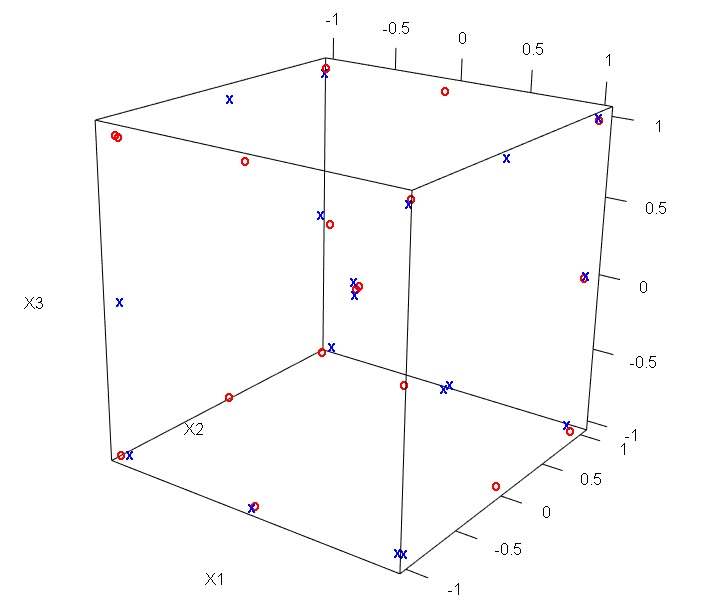
\includegraphics[scale=0.65]{CS_design.jpg}      %width=\textwidth
\caption{MSE(D)-optimal design \#$1$ with two centre points, $\tau^2=1$}
\label{fig::CS_design}
\end{center}
\end{figure} 

Figure \ref{fig::CS_design} provides a graphical representation of the design: the three axes correspond to the experimental factors, each is at three levels (i.e. scaled to $[-1,1]$ dosages): $-1$, $0$ and $1$. Each dot is a design point, and two colours (blue and red) and two symbols (`x' and `o') serve as block indicators. We can see that there are only two centre points in each block, as required, and replicates of other points are generally split between blocks (except for the $(-1,1,1)$ point which is duplicated in the first block only). 

All other designs may be found in the Supplementary material. Time-wise, for the search algorithm's parameters outlined in the beginning of this section, on average an optimal design was found in $13-15$ hours, which was acceptable in this particular case. Sometimes, however, it took up to $20-24$ hours, so some extra time allowance should be accounted for when using these criteria and this search algorithm. 

%%% MSE(D)-optimal designs, WITH centre points: DP, LoF(DPs) and MSE(D) -- LoF as Ds for potential terms
Further we decided to check what designs we would get if there were $5$ levels of each factor rather than $3$, so that all of the third-order terms are estimable (which is also feasible due to a large enough number of runs), i.e. the lack-of-fit component minimising the posterior confidence region for the potential terms would be replaced by the $DP_S$-optimality for them, as in (\ref{eq::crit2}). 

The summary of the corresponding optimal designs is given in Table \ref{tab::MSE(D)_caseCPLoF}: the `new' lack-of-fit component is denoted by DP*s. The notions of `global'  and `local' efficiencies are the same as previously. For each design we calculated its $LoF(DP)$-value, so that we could assess how they would perform in terms of the criterion (\ref{eq::crit1}). The performances of the optimal designs constructed without the restriction of two centre points per block are summarised in Table \ref{tab::MSE(D)_full} in Appendix \ref{app::cs}; all of the designs are also provided in the Supplementary material. In order to illustrate general tendencies in the designs' appearances, designs optimal with respect to the criterion with equal weights, for two values of $\tau^2$ are provided in Table \ref{tab::Full_designs}.

\begin{table}[h]
\centering
\caption{Case-study. Properties of ``Full'' MSE(D)-optimal blocked designs, with two centre points per block}
\label{tab::MSE(D)_caseCPLoF}
\resizebox{\textwidth}{!}}  & \multicolumn{4}{l}{\textbf{`Local' Efficiency,\%}}& \multicolumn{1}{c}{\textbf{Relative}}                          \\
   & \textbf{DP}       & \textbf{DP*s}    & \textbf{MSE(D)}   & \textbf{PE}        & \textbf{LoF}        & \textbf{DP} & \textbf{DP*s}  & \textbf{LoF(DP)}   & \textbf{MSE(D)}  &  \textbf{DP}  &  \textbf{DP*s} & \textbf{LoF(DP)}   & \textbf{MSE(D)} & \textbf{Efficiency,\%} \\
1 & 1/3 & 1/3 & 1/3 & \multicolumn{1}{|r}{14} & \multicolumn{1}{r|}{11} & 80.58 & 69.38 & 87.05 & 91.74 & \multicolumn{1}{|r}{84.46} & 79.90 & 94.36 & \multicolumn{1}{r|}{92.46} & 94.42 \\
2 & 0.4 & 0.2 & 0.4 & \multicolumn{1}{|r}{14} & \multicolumn{1}{r|}{11} & 83.90 & 61.18 & 85.36 & 57.47 & \multicolumn{1}{|r}{87.93} & 70.46 & 92.52 & \multicolumn{1}{r|}{57.92} & 95.83 \\
3 & 0.25 & 0.25 & 0.5 & \multicolumn{1}{|r}{13} & \multicolumn{1}{r|}{12} & 79.93 & 68.24 & 87.06 & 94.05 & \multicolumn{1}{|r}{83.77} & 78.59 & 94.37 & \multicolumn{1}{r|}{94.79} & 96.32 \\
4 & 1 & 0 & 0 & \multicolumn{1}{|r}{20} & \multicolumn{1}{r|}{5} & 95.41 & 0.00 & 62.13 & 95.24 & \multicolumn{1}{|r}{100.00} & 0.00 & 67.34 & \multicolumn{1}{r|}{95.98} & 95.41 \\
5 & 0 & 1 & 0 & \multicolumn{1}{|r}{14} & \multicolumn{1}{r|}{11} & 62.01 & 86.83 & 92.98 & 74.95 & \multicolumn{1}{|r}{64.99} & 100.00 & 100.78 & \multicolumn{1}{r|}{75.53} & 86.83 \\
6 & 0 & 0 & 1 & \multicolumn{1}{|r}{14} & \multicolumn{1}{r|}{11} & 88.31 & 0.00 & 88.35 & 99.23 & \multicolumn{1}{|r}{92.55} & 0.00 & 95.77 & \multicolumn{1}{r|}{100.00} & 99.23 \\
 & & & & & & & & & & & & & & \\
   & \multicolumn{3}{l}{\textbf{Criteria, $\bm{\tau^2=1/q}$}} & \multicolumn{2}{l}{\textbf{DoF}} & \multicolumn{4}{l}{\textbf{`Global' Efficiency,\%}}  & \multicolumn{4}{l}{\textbf{`Local' Efficiency,\%}}& \multicolumn{1}{c}{\textbf{Relative}}                          \\
    & \textbf{DP}       & \textbf{DP*s}    & \textbf{MSE(D)}   & \textbf{PE}   & \textbf{LoF}        & \textbf{DP} & \textbf{DP*s}  & \textbf{LoF(DP)}   & \textbf{MSE(D)}  &  \textbf{DP} & \textbf{DP*s} & \textbf{LoF(DP)}   & \textbf{MSE(D)} & \textbf{Efficiency,\%} \\
1 & 1/3 & 1/3 & 1/3 & \multicolumn{1}{|r}{14} & \multicolumn{1}{r|}{11} & 80.14 & 69.01 & 87.70 & 91.41 & \multicolumn{1}{|r}{83.99} & 81.43 & 90.34 & \multicolumn{1}{r|}{92.07} & 93.97\\
2 & 0.4 & 0.2 & 0.4 & \multicolumn{1}{|r}{14} & \multicolumn{1}{r|}{11} & 83.76 & 61.29 & 88.28 & 94.41 & \multicolumn{1}{|r}{87.79} & 72.31 & 90.95 & \multicolumn{1}{r|}{95.09} & 96.04\\
3 & 0.25 & 0.25 & 0.5 & \multicolumn{1}{|r}{12} & \multicolumn{1}{r|}{13} & 79.66 & 64.43 & 84.44 & 94.84 & \multicolumn{1}{|r}{83.49} & 76.02 & 86.99 & \multicolumn{1}{r|}{95.52} & 95.20\\
4 & 1 & 0 & 0 & \multicolumn{1}{|r}{20} & \multicolumn{1}{r|}{5} & 95.41 & 0.00 & 90.63 & 95.66 & \multicolumn{1}{|r}{100.00} & 0.00 & 93.37 & \multicolumn{1}{r|}{96.35} &  95.41\\
5 & 0 & 1 & 0 & \multicolumn{1}{|r}{14} & \multicolumn{1}{r|}{11} & 59.81 & 84.75 & 86.15 & 72.05 & \multicolumn{1}{|r}{62.68} & 100.00 & 88.75 & \multicolumn{1}{r|}{72.57} & 84.75 \\
6 & 0 & 0 & 1 & \multicolumn{1}{|r}{14} & \multicolumn{1}{r|}{11} & 88.73 & 0.00 & 90.57 & 99.29 & \multicolumn{1}{|r}{92.99} & 0.00 & 93.30 & \multicolumn{1}{r|}{100.00} & 99.29
\end{tabular}
}
\end{table}

\begin{table}[h]
\centering
\caption{Case-study. Designs \#$1$ from Table \ref{tab::MSE(D)_caseCPLoF}, $\tau^2=1$ (left) and $\tau^2=1/q$ (right)}
\begin{center}
\label{tab::Full_designs}
\scalebox{0.73}{
\begin{tabular}{rrrrrrrr|r|rrrrlrrr}
-1 & -1 & 0 &  & -1 & -1 & -1 &  &  &  & -1 & -1 & -1 &  & -1 & -1 & -1 \\
-1 & -1 & 1 &  & -1 & -1 & 0 &  &  &  & -1 & -1 & 0.5 &  & -1 & -1 & 0.5 \\
-1 & 0 & -1 &  & -1 & -1 & 1 &  &  &  & -1 & -0.5 & 1 &  & -1 & -0.5 & 1 \\
-1 & 0.5 & 1 &  & -1 & 0.5 & 1 &  &  &  & -1 & 0 & -0.5 &  & -1 & 1 & -1 \\
-1 & 1 & -1 &  & -1 & 1 & -1 &  &  &  & -1 & 1 & -1 &  & -1 & 1 & 1 \\
-1 & 1 & 0.5 &  & -1 & 1 & 0.5 &  &  &  & -1 & 1 & 1 &  & -0.5 & -1 & -0.5 \\
-0.5 & 1 & 1 &  & -0.5 & -0.5 & 1 &  &  &  & -0.5 & 1 & 0 &  & -0.5 & 0.5 & -1 \\
0 & -1 & -1 &  & -0.5 & 1 & -0.5 &  &  &  & 0 & -1 & 1 &  & 0 & -1 & 1 \\
0 & 0 & 0 &  & 0 & -1 & -1 &  &  &  & 0 & 0 & 0 &  & 0 & 0 & 0 \\
0 & 0 & 0 &  & 0 & 0 & 0 &  &  &  & 0 & 0 & 0 &  & 0 & 0 & 0 \\
0.5 & -1 & 1 &  & 0 & 0 & 0 &  &  &  & 0 & 1 & 1 &  & 0 & 1 & 1 \\
0.5 & 1 & -1 &  & 0.5 & -1 & 1 &  &  &  & 0.5 & -0.5 & -1 &  & 0.5 & 1 & -0.5 \\
1 & -1 & -1 &  & 0.5 & 1 & -1 &  &  &  & 1 & -1 & -1 &  & 1 & -1 & -1 \\
1 & -1 & 0.5 &  & 1 & -1 & -1 &  &  &  & 1 & -1 & 0 &  & \textbf{1} & \textbf{-1} & \textbf{1} \\
1 & -0.5 & 1 &  & 1 & -1 & 0.5 &  &  &  & 1 & 0.5 & 1 &  & \textbf{1} & \textbf{-1} & \textbf{1} \\
1 & 0.5 & -1 &  & 1 & -0.5 & -0.5 &  &  &  & \textbf{1} & \textbf{1} & \textbf{-1} &  & 1 & 0 & -0.5 \\
1 & 1 & -0.5 &  & 1 & 0.5 & -1 &  &  &  & \textbf{1} & \textbf{1} & \textbf{-1} &  & 1 & 0.5 & 1 \\
1 & 1 & 1 &  & 1 & 1 & 1 &  &  &  & 1 & 1 & 0.5 &  & 1 & 1 & 0.5
\end{tabular}
}
\end{center}
\end{table}

In case of $\tau^2=1$ all pure error degrees of freedom (except for the $2$ coming from the replicated centre points) occur from $12$ points duplicated in different blocks; in case of $\tau^2=1/q$ (i.e. $\tau^2=0.1$) two `corner' points are replicated within the same block (they are highlighted in Table \ref{tab::Full_designs}). Quite a few experimental units would receive an `intermediate' $\pm 0.5$ dosage of at least one product, and as this did not comply with the demands of the experimenters, the choice was still made in favour of the three-level design in Table \ref{tab::CS_Design}. 

%% Discussion points
\section{Conclusions}

In general, this chapter is about exploring the flexibility of the design optimality criteria and implementation introduced previously. We adapted the approach to the framework of a blocked experiment, and by considering an example confirmed some of the key features of the relationships between the individual components, and tendencies in optimal designs obtained with various weight allocation schemes. Due to the relatively high time consumption of the determinant-case criterion calculation, the simplest suggested alternative seemed quite promising in terms of providing adequate designs in a much more reasonable time.

The second part of the chapter is devoted to a real-life design problem, such that the given framework of a blocked factorial experiment with some suspicion regarding possible model disturbance suggested applying the MSE-based criterion for the design construction. In addition, the structure of the criterion and the search algorithm implementation allowed for necessary adaptation with regard to the pre-specified restrictions, so that a set of possible solutions was presented satisfying the objectives of the particular experiment. 

